% !TeX root = ./kernel/easyExam.tex
\section*{Exercice 2 \MarksThree}
\begin{enumerate}
    \item Donnez trois systèmes d'exploitations utilisés dans la mise en place des réseaux intelligents.
    \item Citez deux (02) outils logiciels et quatre (04) outils matériels utilisés
          dans la mise en place d'un réseaux intelligent.
    \item Citez quatre (04) applications des réseaux intelligents.
    \item Donnez quatre (04) des risques encourus par une organisation ayant un réseaux intelligent mal sécurisé ?
    \item Donnez quatre (04) tâches a éffectuer afin de sécuriser les dispositifs des réseaux intelligents ?
    \item Donner deux (02) avantages des réseaux intelligents.
    \item Identifiez et classifier les cartes de la figure \ref{fig:carte} en carte à microcontrôleurs ou en carte à microprocesseur.
\end{enumerate}

\begin{figure}[!ht]
    \centering
    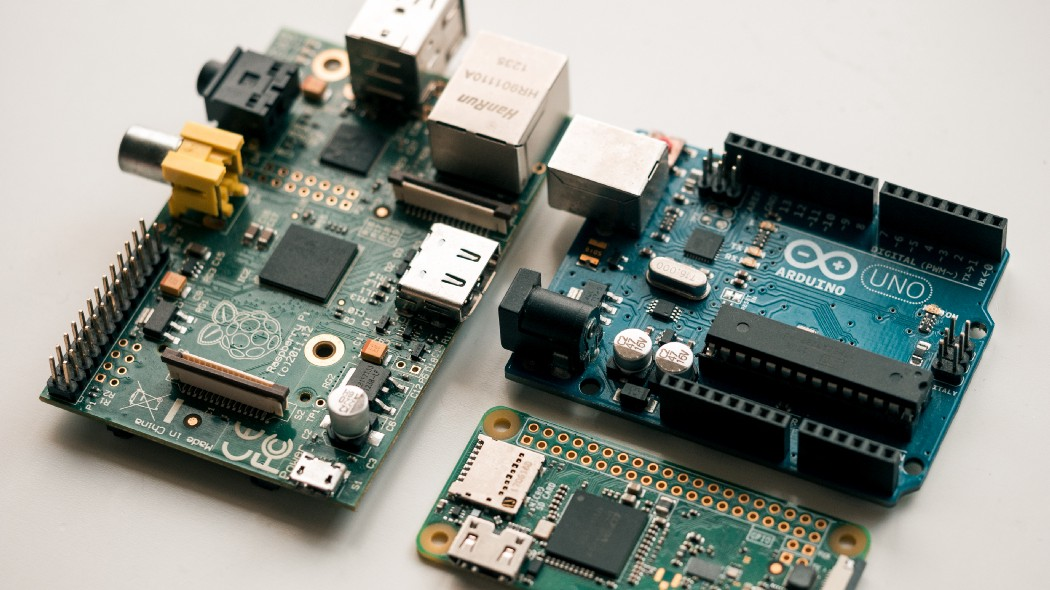
\includegraphics[scale=0.25]{../../figs/hardware_devices.jpg}
    \caption{Quelques cartes pour réseaux intélligents.\label{fig:carte}}
\end{figure}